\documentclass[dvipsnames]{beamer}
\input{mybeamerdefs}

\begin{document}

\begin{frame}{\today}
\begin{itemize}
\item I wrote a script to show that we can simulate the ems in parallel and do the reconstruction afterwards.
\item I tested the execution time of the 2DFT simulation.
\item I tested the execution time of numpy's random number generator.
\item I kept the divorce between the pulse sequence sampling period and the simulation time step but now apply rotation at every simulation time step.
\item I implemented metabolic conversion.
\end{itemize}
\end{frame}

\section{Simulating ems in parallel}

\begin{frame}{Summary}
\begin{itemize}
\item I simulated 2DFT+reconstruction with four ems using the script of 2019-12-11.
\item I ran the same simulation with two of the four ems and stored the MR signals. I repeated the simulation with the other two ems and stored the MR signals. I summed the MR signals and did the reconstruction.
\end{itemize}
\end{frame}

\begin{frame}{4 ems in one run}
\begin{center}
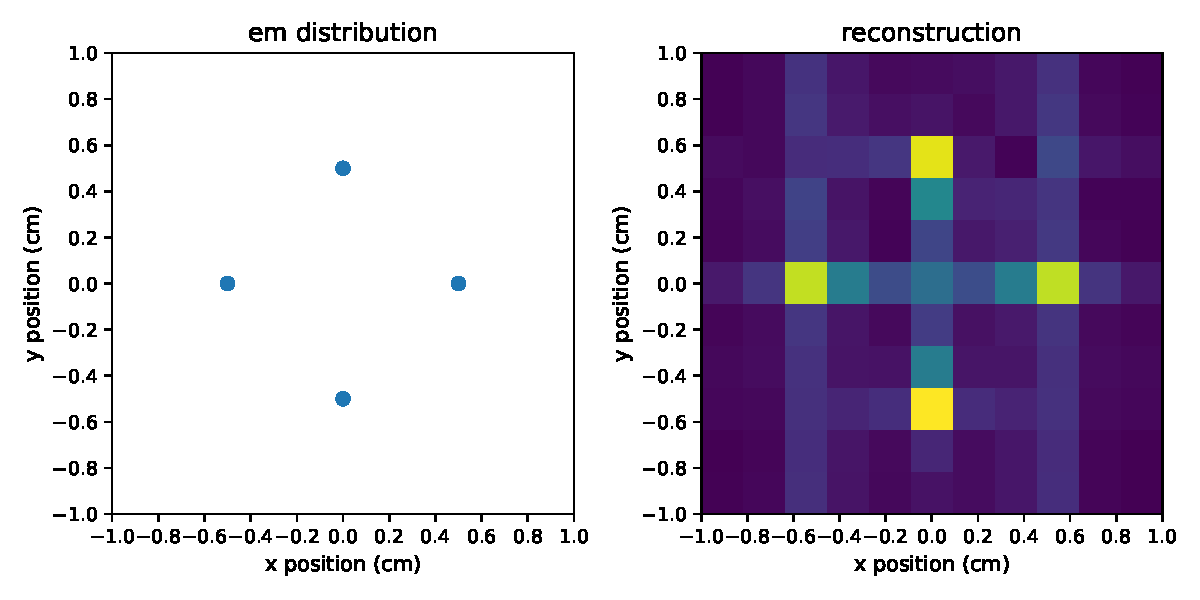
\includegraphics[width=\textwidth]{reconstruction_single}
\end{center}
\end{frame}

\begin{frame}{2 ems in run 1, 2 ems in run 2}
\begin{center}
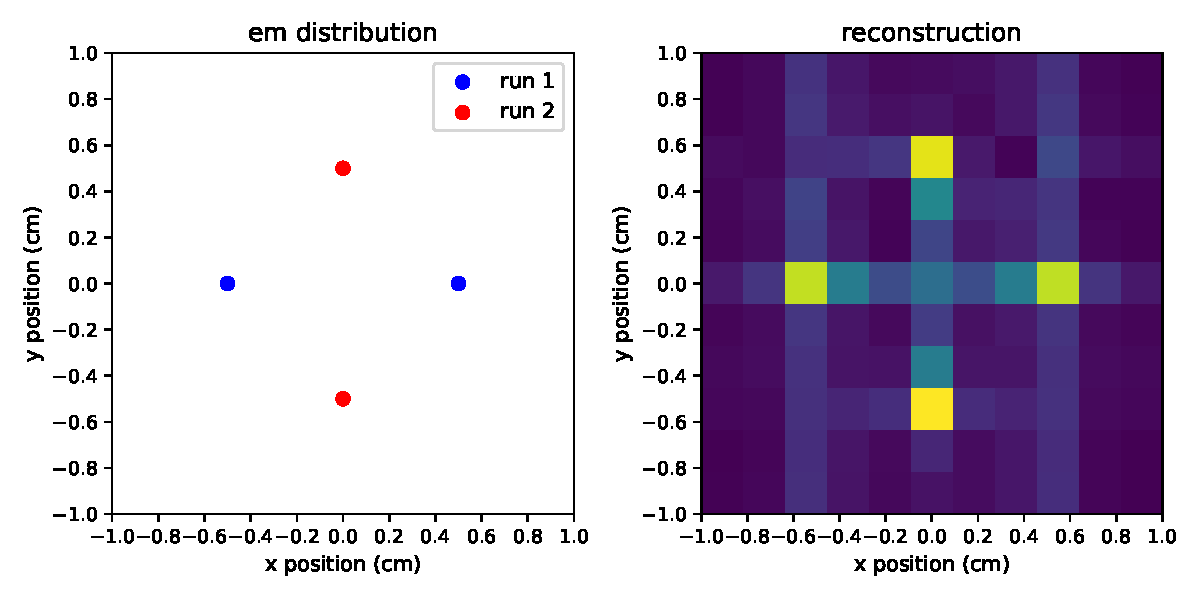
\includegraphics[width=\textwidth]{reconstruction_parallel}
\end{center}
\end{frame}

\begin{frame}{Comments}
\begin{itemize}
\item The reconstructions are identical.
\item We can parallelize the simulation easily. A central computer partitions the ems across the cluster. Each computer simulates its own set of ems and stores the MR signals. Once the simulation is complete, each computer sends the MR signals to the central computer. The central computer does the reconstruction.
\end{itemize}
\end{frame}

\section{Execution time of 2DFT simulation}

\begin{frame}{Summary}
\begin{itemize}
\item I tested the execution time of the 2DFT simulation using one em with 9 TRs of length 111 ms (1 s pulse sequence length) and a time step of 1 us (implying $10^6$ time steps).
\item The total execution time was 5.41 seconds.
\item The execution time is 5.41 us per em per time step.
\end{itemize}
\end{frame}

\section{Execution time of random number generation with Numpy}

\begin{frame}{Summary}
\begin{itemize}
\item Using the command \texttt{numpy.random.random()} to generate a random number between 0.0 and 1.0, I found it took 0.346 seconds to generate 1 million random numbers.
\item This means 0.346 microseconds per random number.
\item This would increase the execution time from 5.41 us to 5.76 us per em per time step (6.5\% increase in execution time).
\end{itemize}
\end{frame}

\section{Metabolic conversion}

\begin{frame}{Summary}
\begin{itemize}
\item I implemented metabolic conversion in the ems.
\item At each simulation time step for each em, a random number in $[0.0,1.0)$ is generated. If this number is less than the conversion probability for the duration of the time step (e.g. 5\% per second $\Rightarrow$ $5 \times 10^{-6}\%$ per microsecond), then the shielding constant of the em is updated.
\end{itemize}
\end{frame}

\begin{frame}{Metabolic conversion off}
\begin{center}
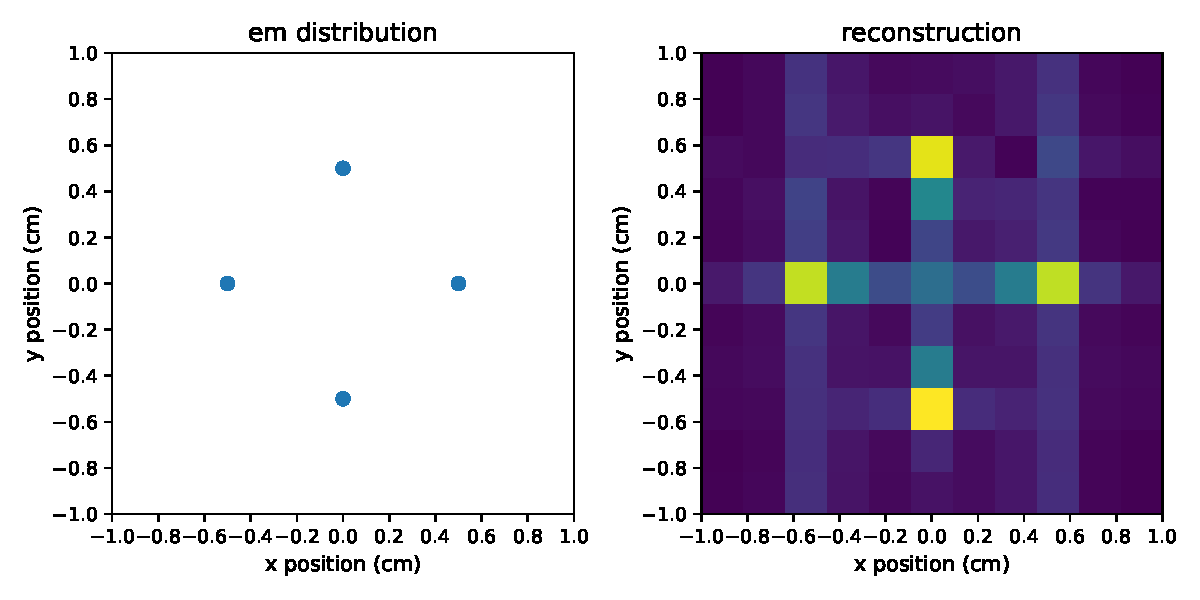
\includegraphics[width=\textwidth]{reconstruction_metabolism-off}
\end{center}
\end{frame}

\begin{frame}{Metabolic conversion on, rate = 20\% per second, chemical shift = 10 ppm}
\begin{center}
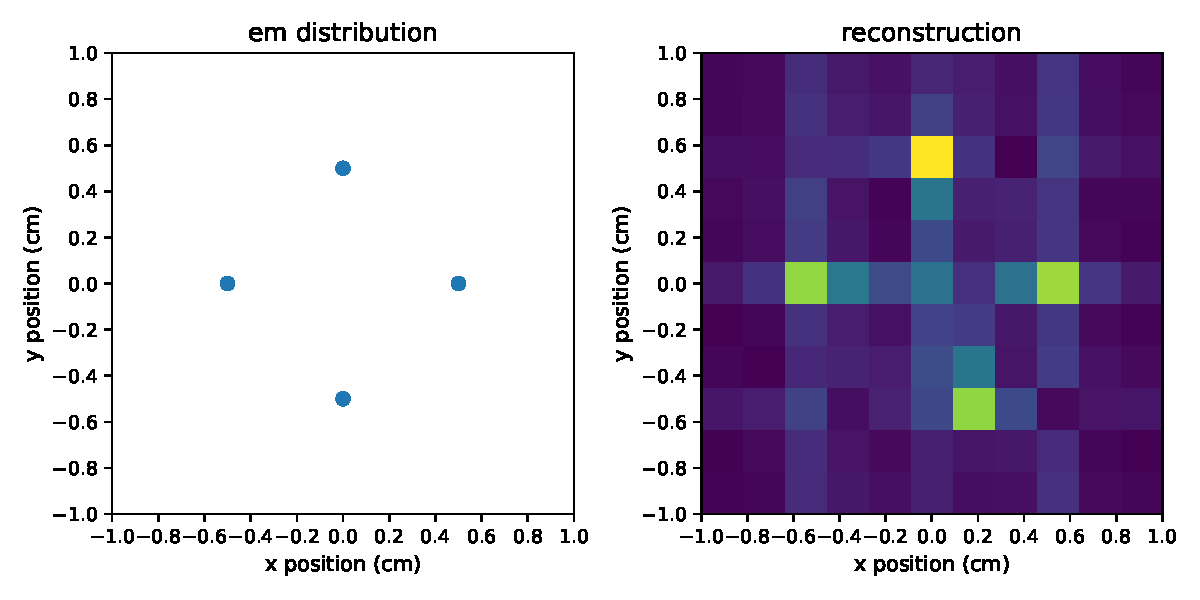
\includegraphics[width=\textwidth]{reconstruction_metabolism-on-20percent}
\end{center}
\end{frame}

\begin{frame}{Comments}
\begin{itemize}
\item The change in resonance frequency distorts the image.
\end{itemize}
\end{frame}

\end{document}